\documentclass[12pt, a4paper]{article}

%include packages
\usepackage{a4}
\usepackage[dvips]{graphicx}
\usepackage[ansinew]{inputenc}
\usepackage{epsfig}
\usepackage{subcaption}
\usepackage{amsmath}
\usepackage{amssymb}

\pagestyle{plain}
\pagenumbering{arabic}

\title{Real Valued Test Functions}
\author{Heuristic and Evolutionary Algorithms Laboratory (HEAL)}
\date{\today}

\begin{document}
	\maketitle

	\section*{Ackley Function}
		\begin{equation*}
			f(x) = 20 + e - 20e^{-\frac{1}{5} \sqrt{\frac{1}{n} \sum_{i=1}^n x_i^2}} - e^{\frac{1}{n} \sum_{i=1}^n \cos(2 \pi x_i)}
		\end{equation*}

		\begin{tabbing}
			\hspace{5cm}\=\kill
			\textbf{Dimensions:}     \> $n$ \\
			\textbf{Domain:}         \> $-32.768 \leq x_i \leq 32.768$ \\
			\textbf{Global Optimum:} \> $f(x) = 0.0$ at $x = (0.0, 0.0, \dots, 0.0)$ \\
			\textbf{Operator:}       \> AckleyEvaluator \\
			\textbf{Charts:}         \> \\
		\end{tabbing}

		\begin{figure}[ht]
			\begin{subfigure}{0.49\textwidth}
				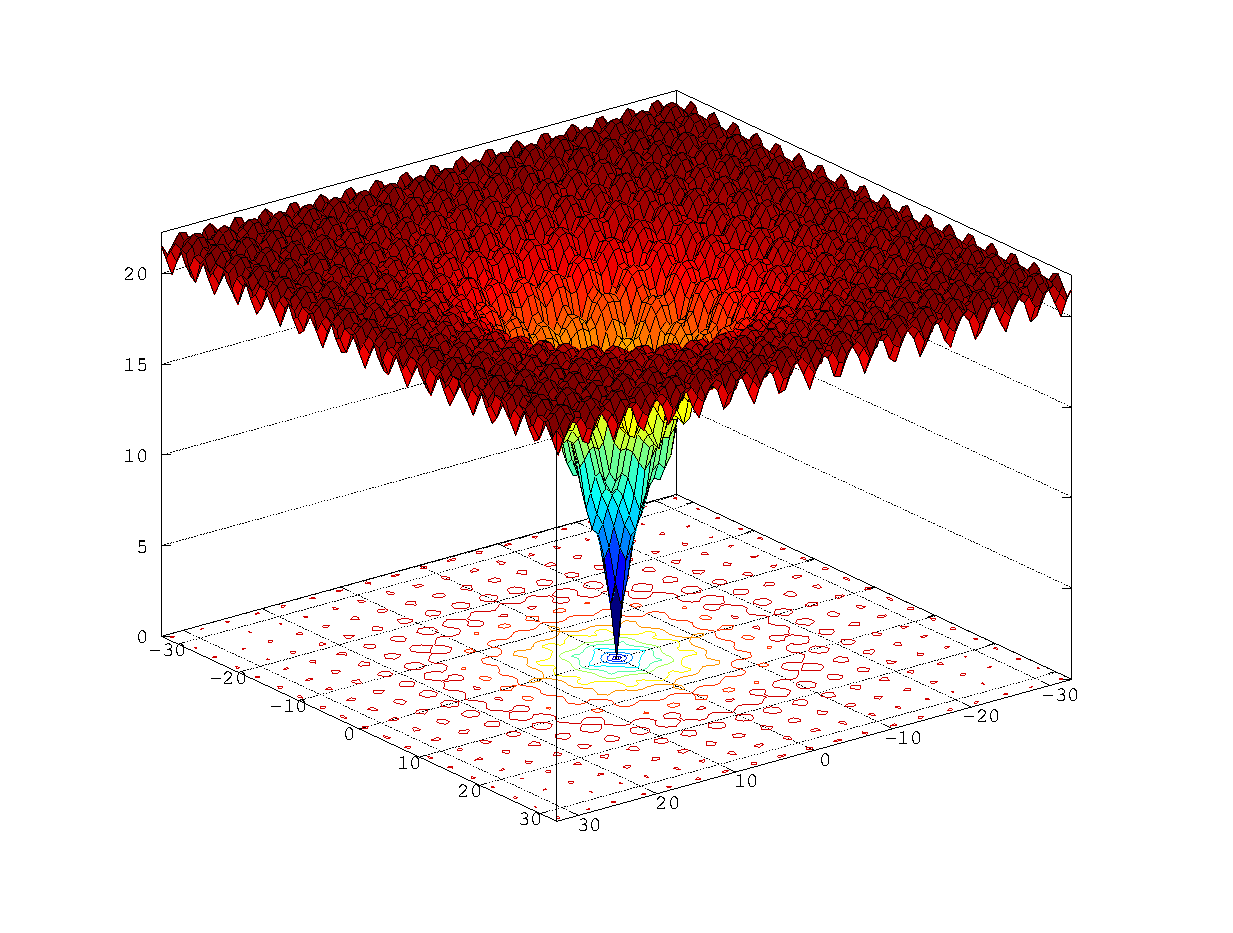
\includegraphics[width=\linewidth]{Images/Ackley_large}
				\caption{[-32.768, 32.768]}
			\end{subfigure}
			\begin{subfigure}{0.49\textwidth}
				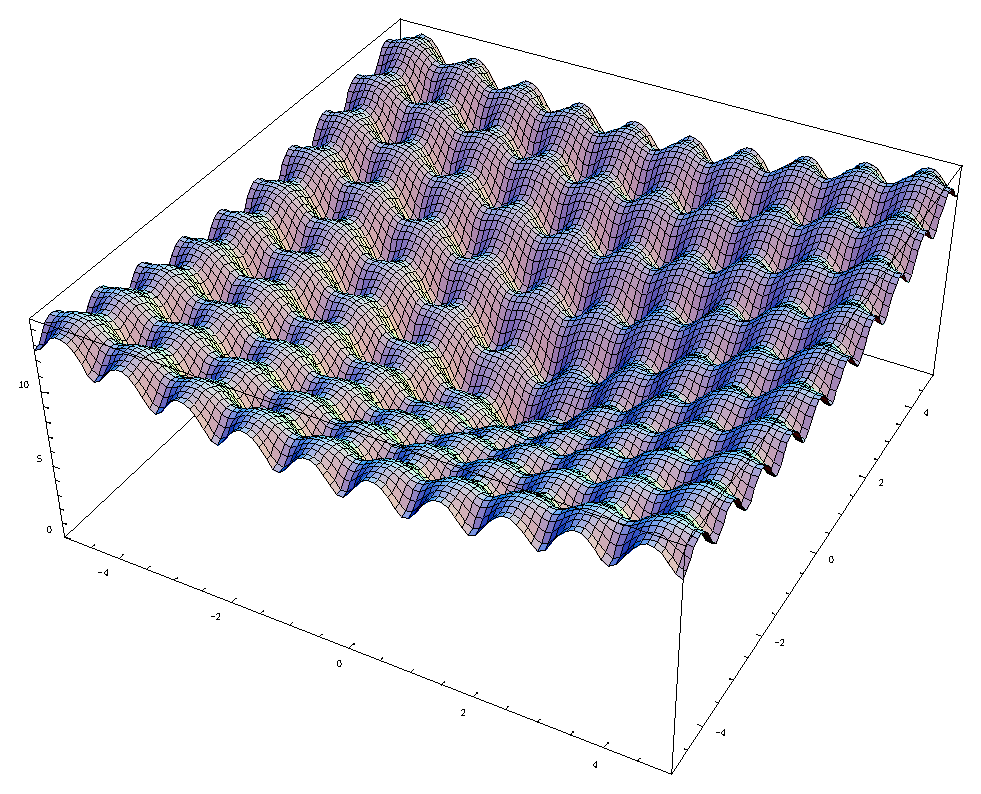
\includegraphics[width=\linewidth]{Images/Ackley_small}
				\caption{[-6.0, 6.0]}
			\end{subfigure}
			\caption{Ackley function plots.}
		\end{figure}

	\newpage

	\section*{Beale Function}
		\begin{equation*}
			f(x)=(1.5-x_1+x_1x_2)^2+(2.25-x_1+x_1x_2^2)^2+(2.625 - x_1 + x_1x_2^3)^2
		\end{equation*}

		\begin{tabbing}
			\hspace{5cm}\=\kill
			\textbf{Dimensions:}     \> $2$ \\
			\textbf{Domain:}         \> $-4.5 \leq x_i \leq 4.5$ \\
			\textbf{Global Optimum:} \> $f(x) = 0.0$ at $x = (3.0, 0.5)$ \\
			\textbf{Operator:}       \> BealeEvaluator \\
			\textbf{Charts:}         \> \\
		\end{tabbing}

		\begin{figure}[ht]
			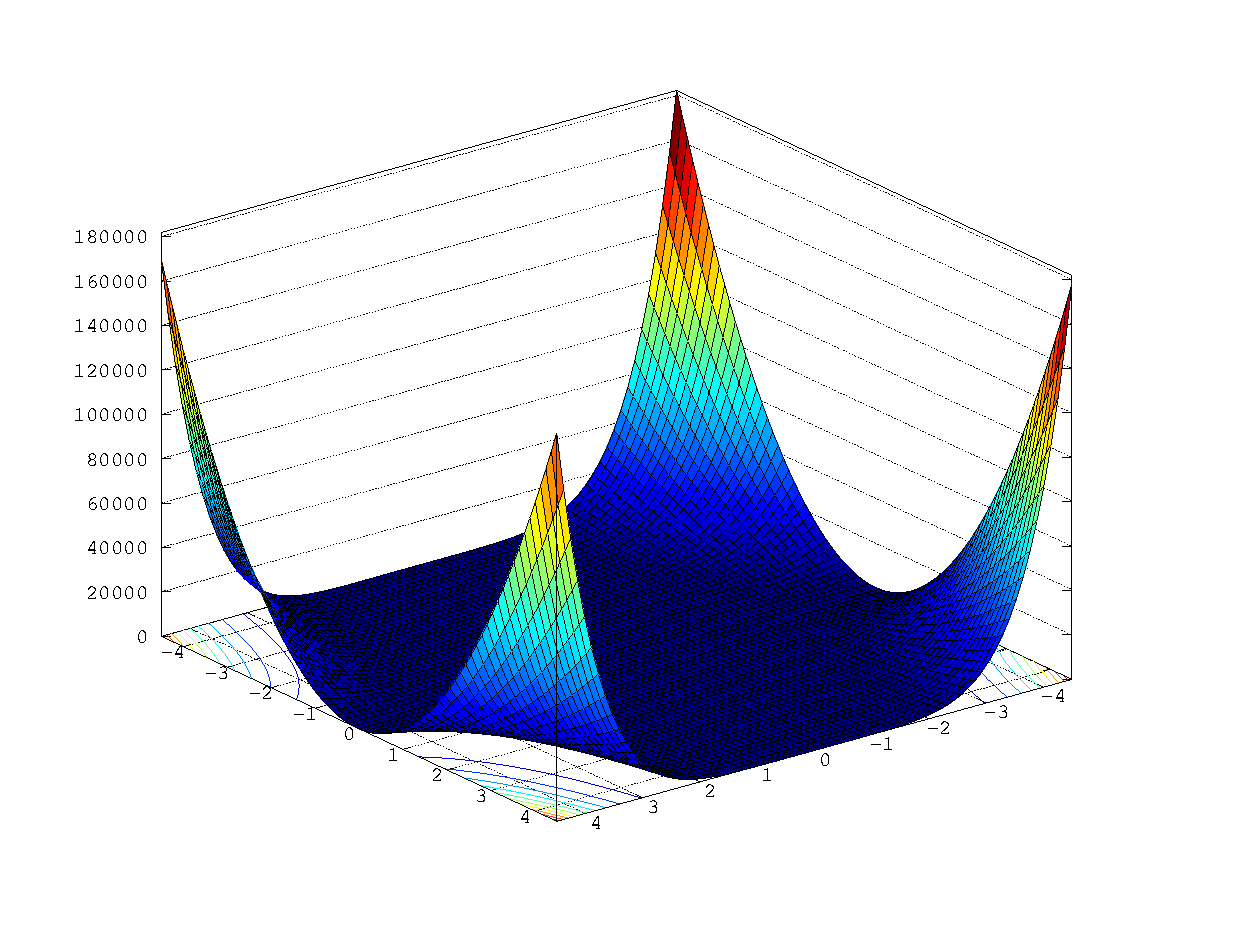
\includegraphics[width=\textwidth]{Images/Beale}
			\caption{Beale function [-4.5, 4.5].}
		\end{figure}

	\newpage

	\section*{Booth Function}
		\begin{equation*}
			f(x)=(x_1+2x_2-7)^2+(2x_1+x_2-5)^2
		\end{equation*}

		\begin{tabbing}
			\hspace{5cm}\=\kill
			\textbf{Dimensions:}     \> $2$ \\
			\textbf{Domain:}         \> $-10.0 \leq x_i \leq 10.0$ \\
			\textbf{Global Optimum:} \> $f(x) = 0.0$ at $x = (1.0, 3.0)$ \\
			\textbf{Operator:}       \> BoothEvaluator \\
			\textbf{Charts:}         \> \\
		\end{tabbing}

		\begin{figure}[ht]
			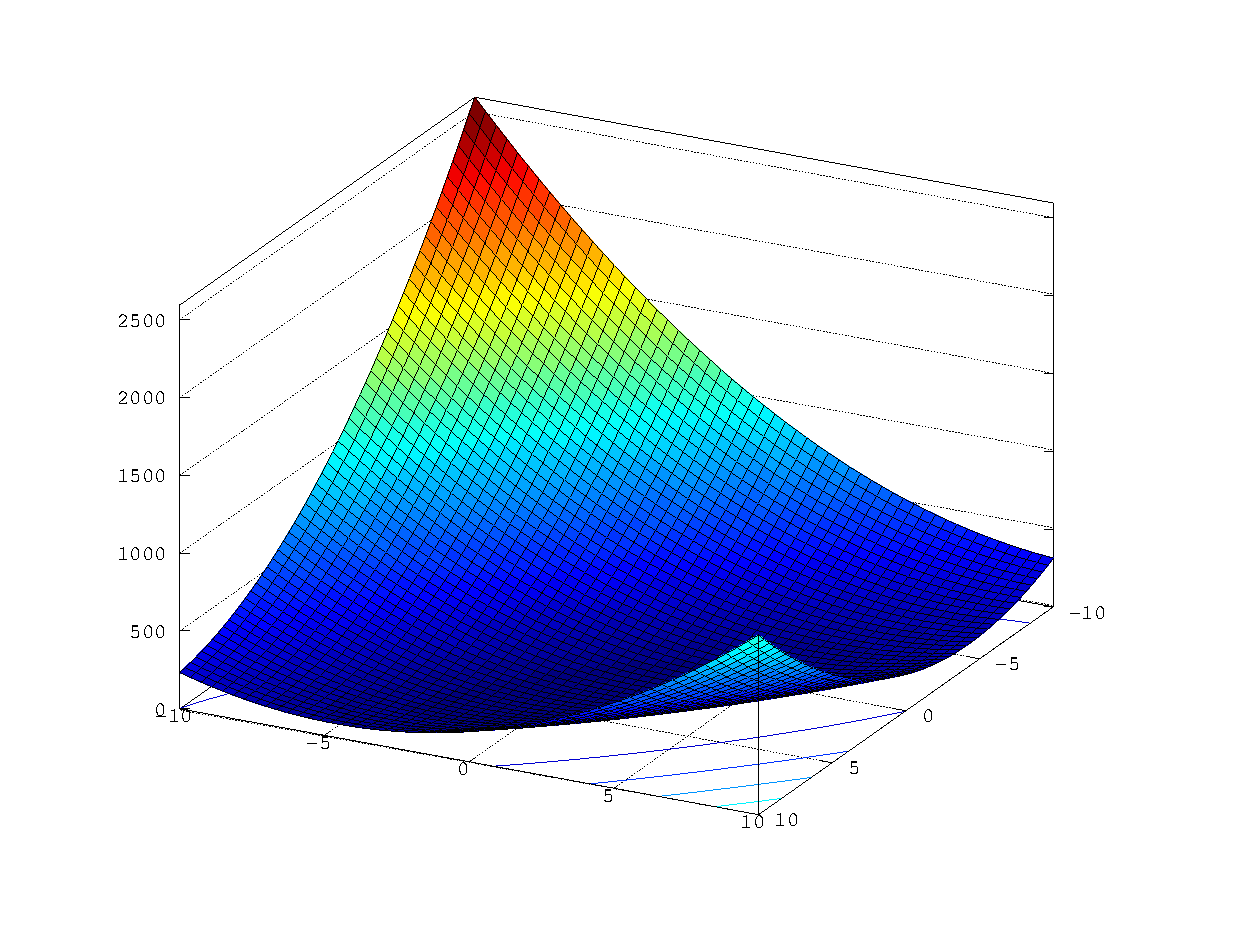
\includegraphics[width=\textwidth]{Images/Booth}
			\caption{Booth function [-10.0, 10.0].}
		\end{figure}

	\newpage

	\section*{Griewank Function}
		\begin{equation*}
			f(x) = 1 + \sum_{i=1}^n \frac{x_i^2}{4000} - \prod_{i=1}^n \cos(\frac{x_i}{\sqrt i})
		\end{equation*}

		\begin{tabbing}
			\hspace{5cm}\=\kill
			\textbf{Dimensions:}     \> $n$ \\
			\textbf{Domain:}         \> $-600.0 \leq x_i \leq 600.0$ \\
			\textbf{Global Optimum:} \> $f(x) = 0.0$ at $x = (0.0, 0.0, \dots, 0.0)$ \\
			\textbf{Operator:}       \> GriewankEvaluator \\
			\textbf{Charts:}         \> \\
		\end{tabbing}

		\begin{figure}[ht]
			\begin{subfigure}{0.49\textwidth}
				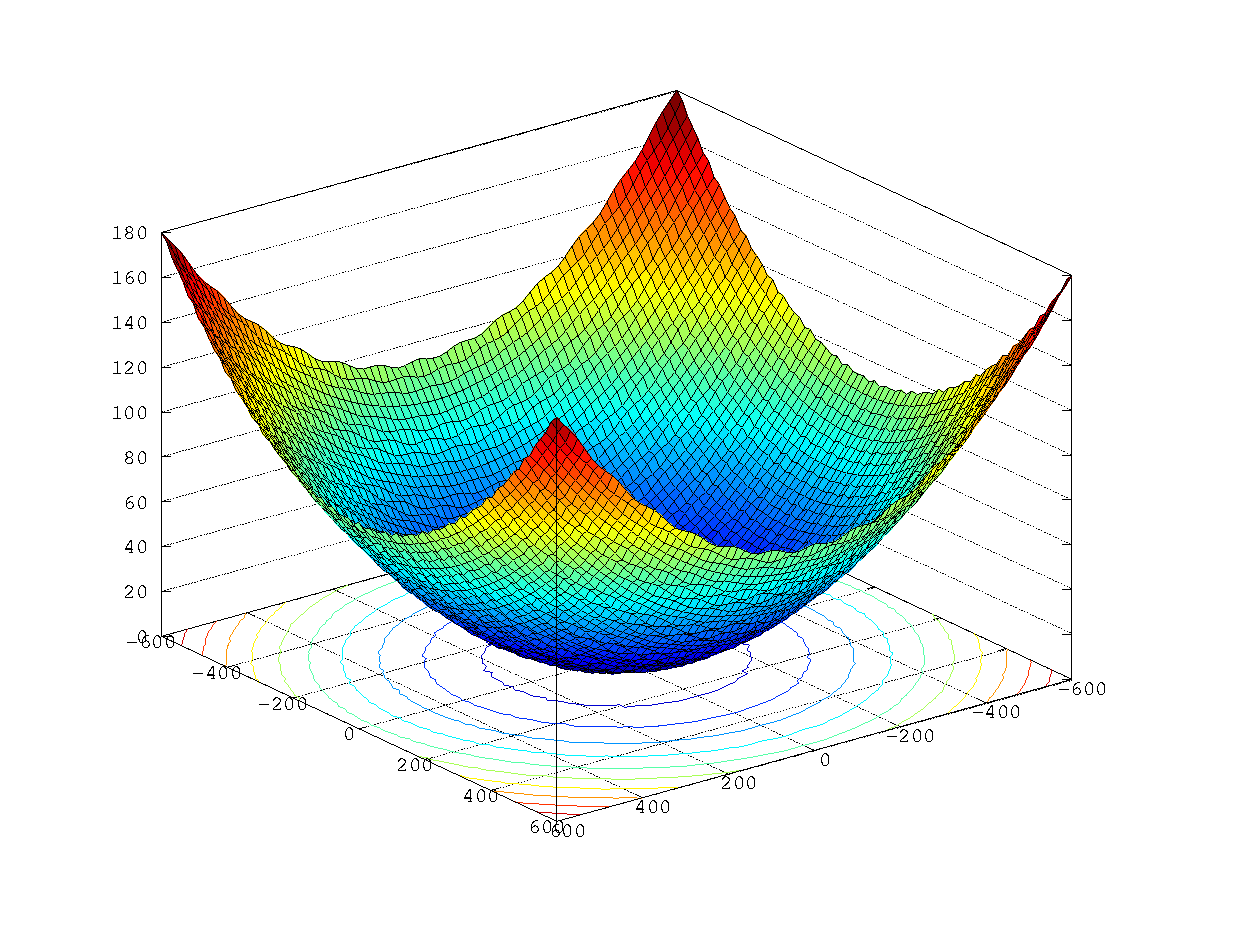
\includegraphics[width=\linewidth]{Images/Griewank_large}
				\caption{[-600.0, 600.0]}
			\end{subfigure}
			\begin{subfigure}{0.49\textwidth}
				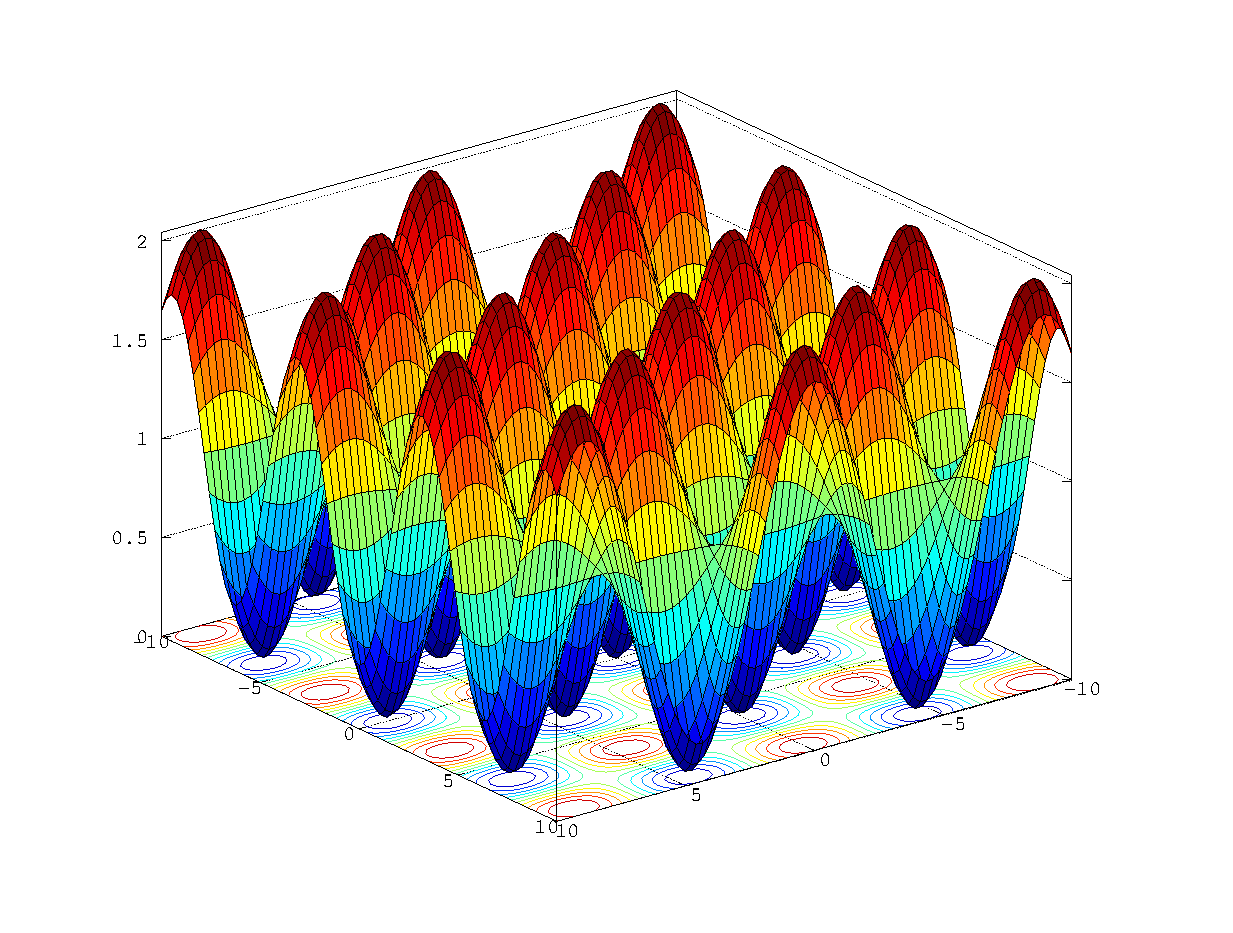
\includegraphics[width=\linewidth]{Images/Griewank_small}
				\caption{[-10.0, 10.0]}
			\end{subfigure}
			\caption{Griewank function plots.}
		\end{figure}

	\newpage

	\section*{Levy Function}
		\begin{equation*}
			f(x)=\sin^2(\pi w_1)+\sum\limits_{i=1}^{n-1}(w_i-1)^2[1+10\sin^2(\pi w_i+1)]+(w_n-1)^2[1+\sin^2(2\pi w_n)]
		\end{equation*}
		\begin{equation*}
			w_i=1+\frac{x_i - 1}{4}, i=1,\dots,n
		\end{equation*}

		\begin{tabbing}
			\hspace{5cm}\=\kill
			\textbf{Dimensions:}     \> $n$ \\
			\textbf{Domain:}         \> $-10.0 \leq x_i \leq 10.0$ \\
			\textbf{Global Optimum:} \> $f(x) = 0.0$ at $x = (1.0, 1.0)$ \\
			\textbf{Operator:}       \> LevyEvaluator \\
			\textbf{Charts:}         \> \\
		\end{tabbing}

		\begin{figure}[ht]
			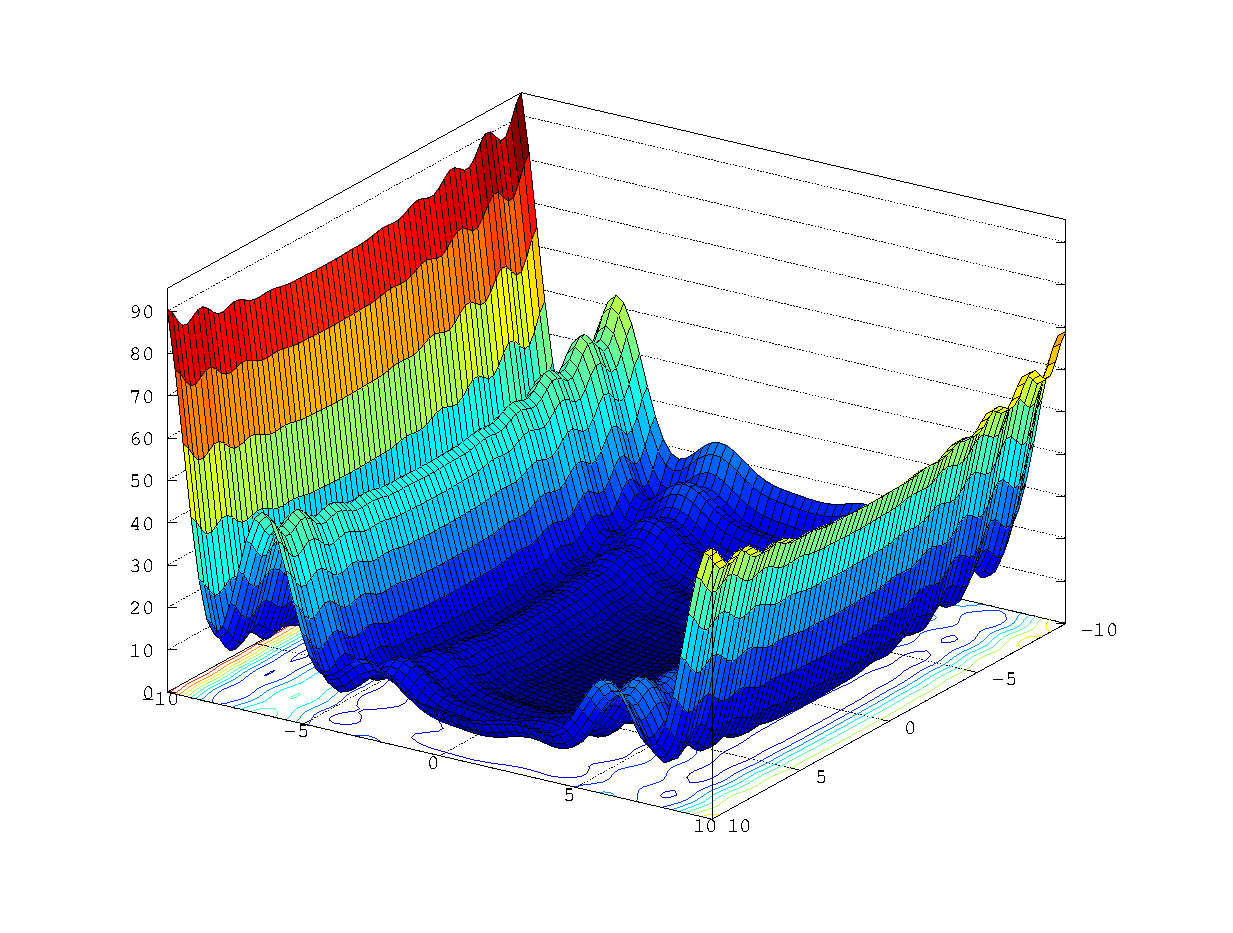
\includegraphics[width=\textwidth]{Images/Levy}
			\caption{Levy function [-10.0, 10.0].}
		\end{figure}

	\newpage

	\section*{Matyas Function}
		\begin{equation*}
			f(x)=0.26(x_1^2+x_2^2)-0.48x_1x_2
		\end{equation*}

		\begin{tabbing}
			\hspace{5cm}\=\kill
			\textbf{Dimensions:}     \> $2$ \\
			\textbf{Domain:}         \> $-10.0 \leq x_i \leq 10.0$ \\
			\textbf{Global Optimum:} \> $f(x) = 0.0$ at $x = (0.0, 0.0)$ \\
			\textbf{Operator:}       \> MatyasEvaluator \\
			\textbf{Charts:}         \> \\
		\end{tabbing}

		\begin{figure}[ht]
			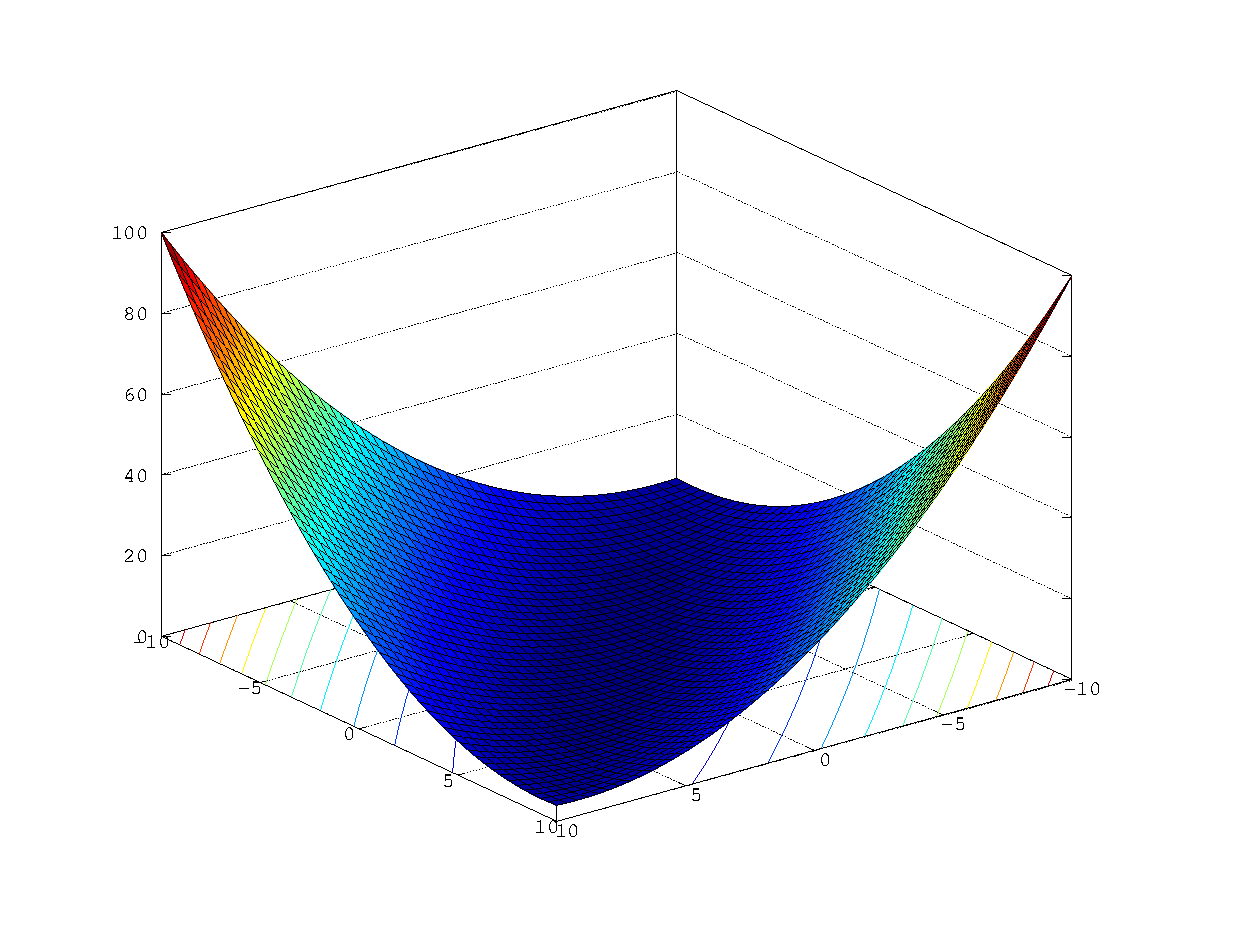
\includegraphics[width=\textwidth]{Images/Matyas}
			\caption{Matyas function [-10.0, 10.0].}
		\end{figure}

	\newpage

	\section*{Rastrigin Function}
		\begin{equation*}
			f(x)=10n+\sum\limits_{i=1}^n[x_i^2-10\cos(2\pi x_i)]
		\end{equation*}

		\begin{tabbing}
			\hspace{5cm}\=\kill
			\textbf{Dimensions:}     \> $n$ \\
			\textbf{Domain:}         \> $-5.12 \leq x_i \leq 5.12$ \\
			\textbf{Global Optimum:} \> $f(x) = 0.0$ at $x = (0.0, 0.0, \dots, 0.0)$ \\
			\textbf{Operator:}       \> RastriginEvaluator \\
			\textbf{Charts:}         \> \\
		\end{tabbing}

		\begin{figure}[ht]
			\begin{subfigure}{0.49\textwidth}
				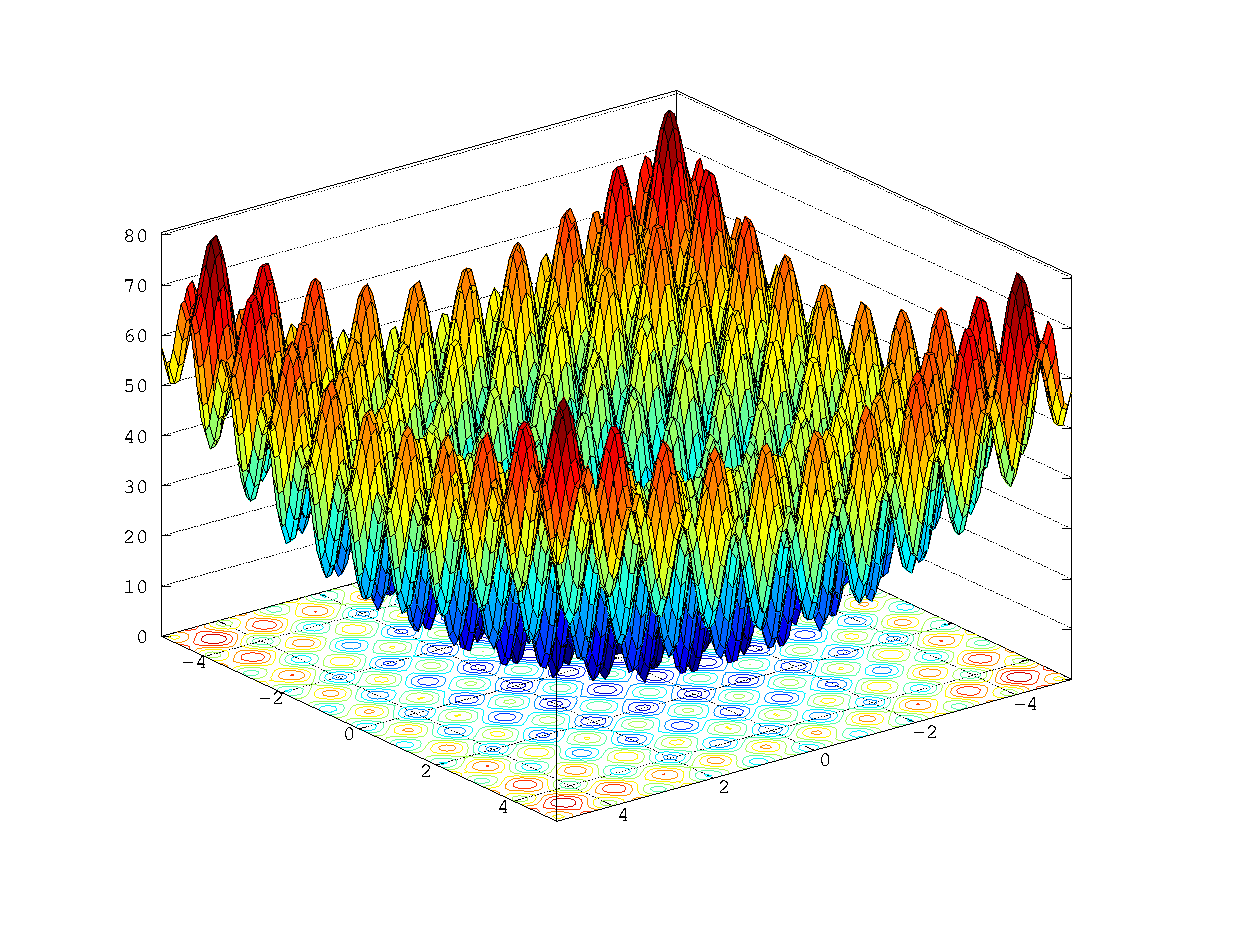
\includegraphics[width=\linewidth]{Images/Rastrigin_large}
				\caption{[-5.12, 5.12]}
			\end{subfigure}
			\begin{subfigure}{0.49\textwidth}
				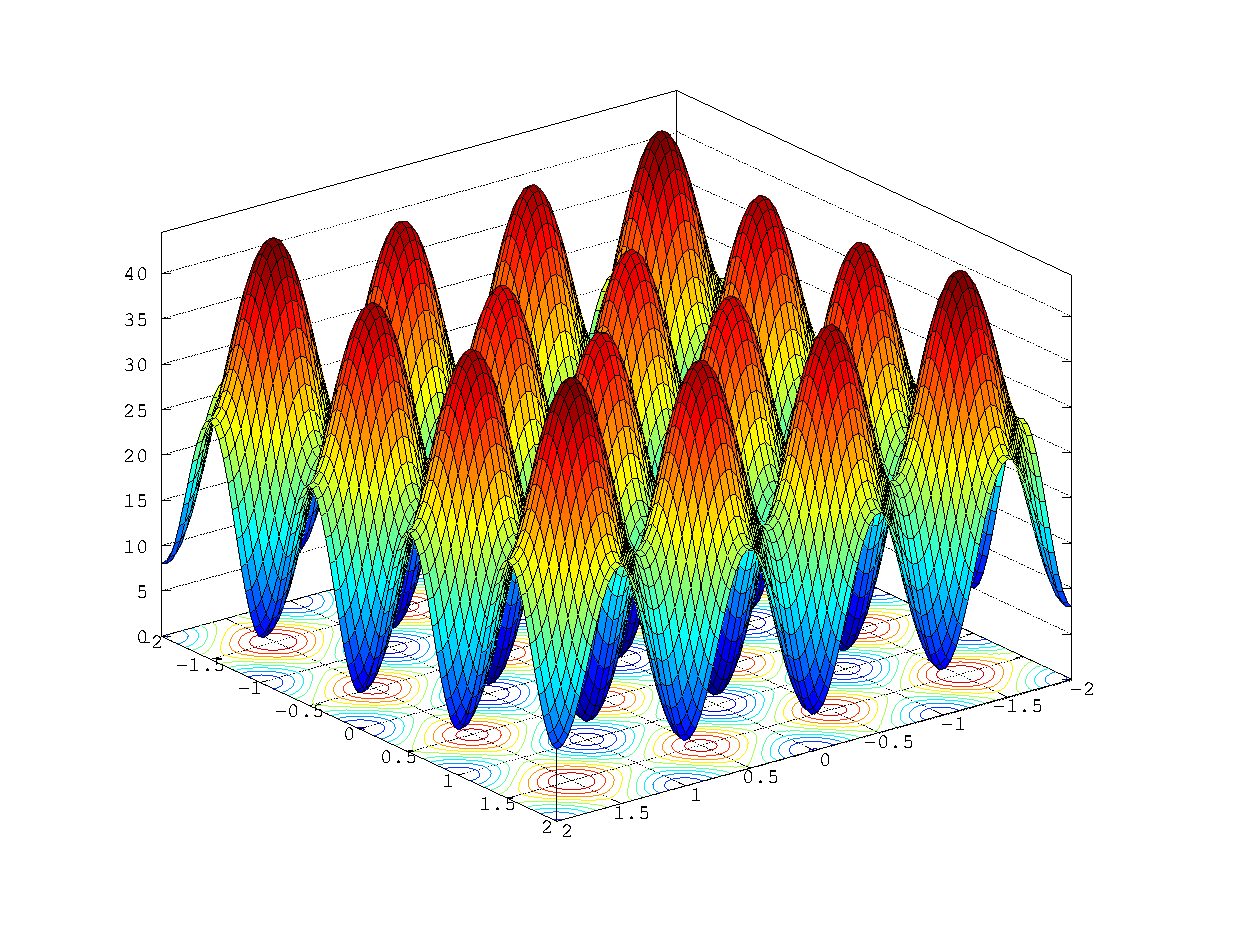
\includegraphics[width=\linewidth]{Images/Rastrigin_small}
				\caption{[-2.0, 2.0]}
			\end{subfigure}
			\caption{Rastrigin function plots.}
		\end{figure}

	\newpage

	\section*{Rosenbrock Function}
		\begin{equation*}
			f(x)=\sum\limits_{i=1}^{n-1}[100(x_i^2-x_{i+1})^2+(x_i-1)^2]
		\end{equation*}

		\begin{tabbing}
			\hspace{5cm}\=\kill
			\textbf{Dimensions:}     \> $n$ \\
			\textbf{Domain:}         \> $-2.048 \leq x_i \leq 2.048$ \\
			\textbf{Global Optimum:} \> $f(x) = 0.0$ at $x = (1.0, 1.0, \dots, 1.0)$ \\
			\textbf{Operator:}       \> RosenbrockEvaluator \\
			\textbf{Charts:}         \> \\
		\end{tabbing}

		\begin{figure}[ht]
			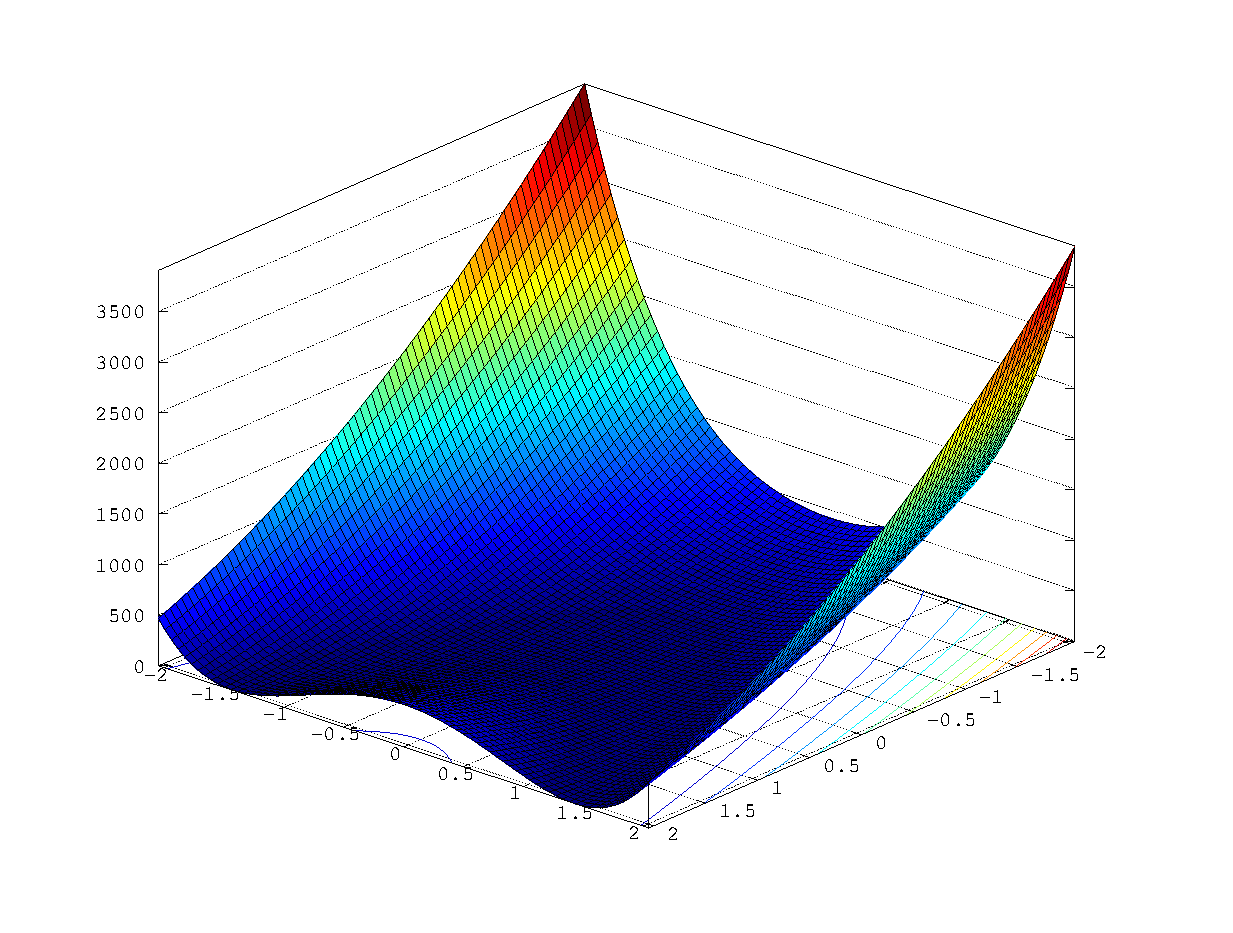
\includegraphics[width=\textwidth]{Images/Rosenbrock}
			\caption{Rosenbrock function [-2.048, 2.048].}
		\end{figure}

	\newpage

	\section*{Schwefel Function}
		\begin{equation*}
			f(x)=418.982887272433n - \sum\limits_{i=1}^n x_i\sin(\sqrt{|x_i|})
		\end{equation*}

		\begin{tabbing}
			\hspace{5cm}\=\kill
			\textbf{Dimensions:}     \> $n$ \\
			\textbf{Domain:}         \> $-500.0 \leq x_i \leq 500.0$ \\
			\textbf{Global Optimum:} \> $f(x) \approx 0.0$ at $x = (420.9687, 420.9687, \dots, 420.9687)$ \\
			\textbf{Operator:}       \> SchwefelEvaluator \\
			\textbf{Charts:}         \> \\
		\end{tabbing}

		\begin{figure}[ht]
			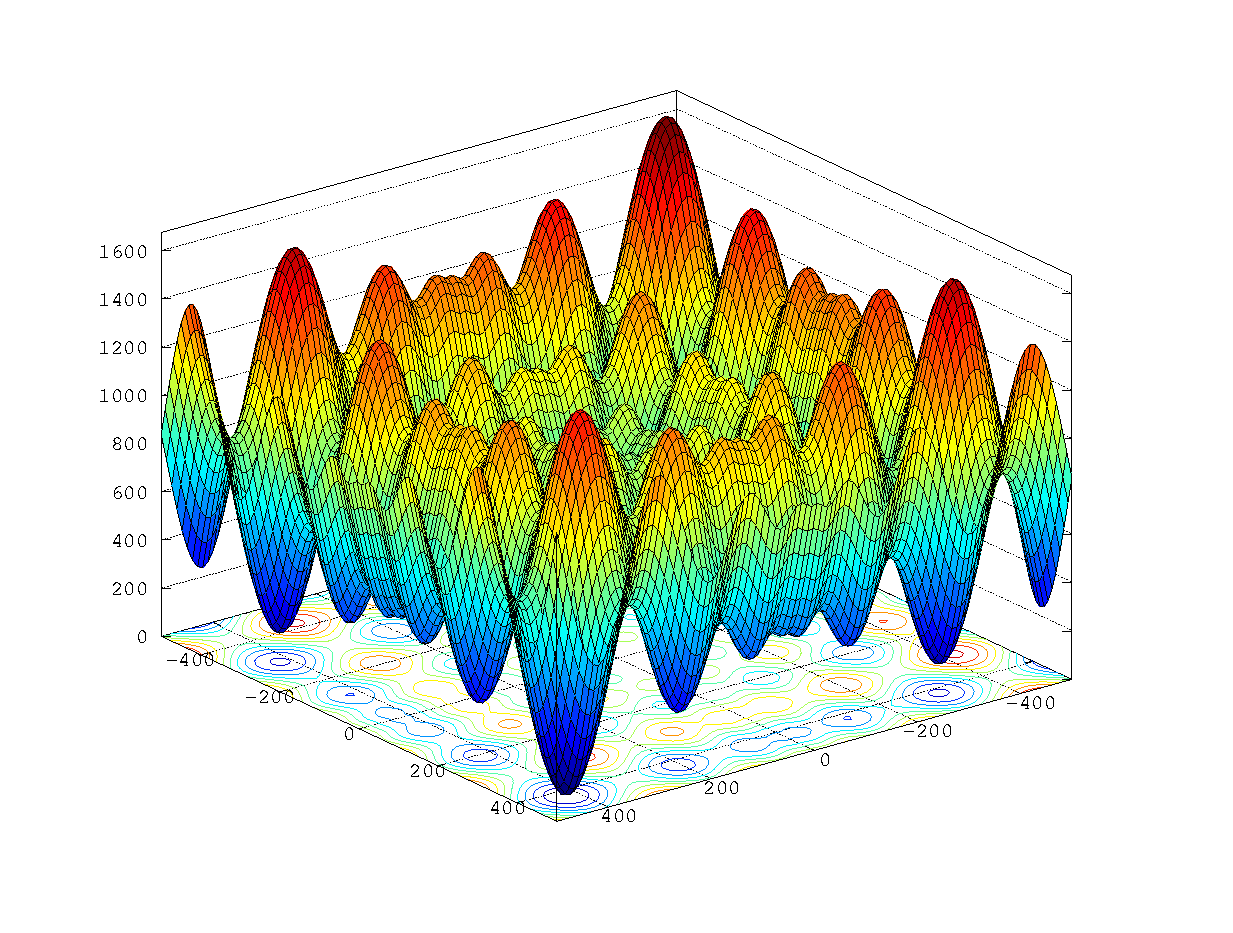
\includegraphics[width=\textwidth]{Images/Schwefel}
			\caption{Schwefel function [-500.0, 500.0].}
		\end{figure}

	\newpage

	\section*{Sphere Function}
		\begin{equation*}
			f(x)=\sum\limits_{i=1}^n x_i^2
		\end{equation*}

		\begin{tabbing}
			\hspace{5cm}\=\kill
			\textbf{Dimensions:}     \> $n$ \\
			\textbf{Domain:}         \> $-5.12 \leq x_i \leq 5.12$ \\
			\textbf{Global Optimum:} \> $f(x) = 0.0$ at $x = (0.0, 0.0, \dots, 0.0)$ \\
			\textbf{Operator:}       \> SphereEvaluator \\
			\textbf{Charts:}         \> \\
		\end{tabbing}

		\begin{figure}[ht]
			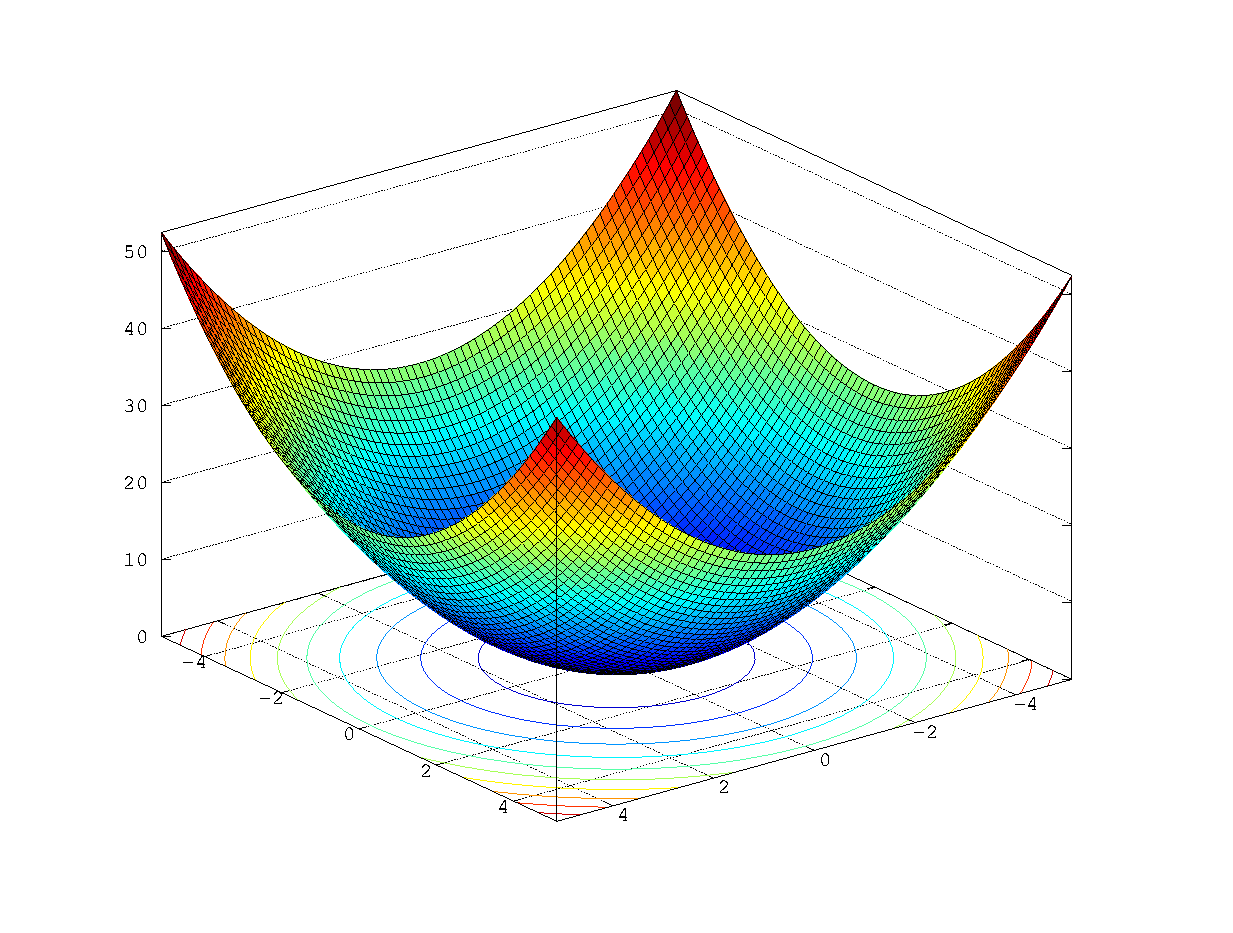
\includegraphics[width=\textwidth]{Images/Sphere}
			\caption{Sphere function [-5.12, 5.12].}
		\end{figure}

	\newpage

	\section*{Sum Squares Function}
		\begin{equation*}
			f(x)=\sum\limits_{i=1}^n ix_i^2
		\end{equation*}

		\begin{tabbing}
			\hspace{5cm}\=\kill
			\textbf{Dimensions:}     \> $n$ \\
			\textbf{Domain:}         \> $-10.0 \leq x_i \leq 10.0$ \\
			\textbf{Global Optimum:} \> $f(x) = 0.0$ at $x = (0.0, 0.0, \dots, 0.0)$ \\
			\textbf{Operator:}       \> SumSquaresEvaluator \\
			\textbf{Charts:}         \> \\
		\end{tabbing}

		\begin{figure}[ht]
			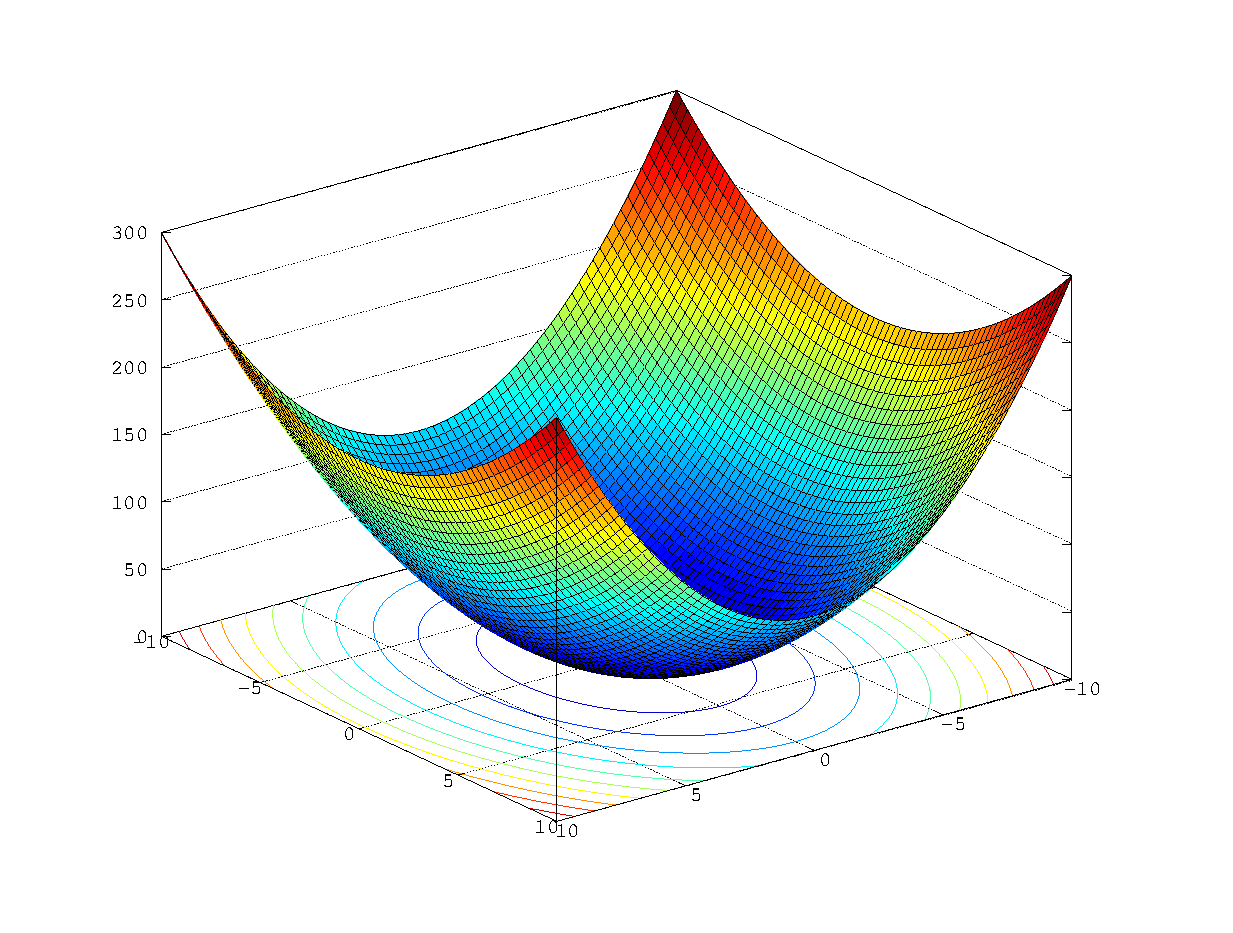
\includegraphics[width=\textwidth]{Images/SumSquares}
			\caption{Sum squares function [-10.0, 10.0].}
		\end{figure}

	\newpage

	\section*{Zakharov Function}
		\begin{equation*}
			f(x)=\sum\limits_{i=1}^n x_i^2+\left(\sum\limits_{i=1}^n 0.5ix_i\right)^2+\left(\sum\limits_{i=1}^n 0.5ix_i\right)^4
		\end{equation*}

		\begin{tabbing}
			\hspace{5cm}\=\kill
			\textbf{Dimensions:}     \> $n$ \\
			\textbf{Domain:}         \> $-5.0 \leq x_i \leq 10.0$ \\
			\textbf{Global Optimum:} \> $f(x) = 0.0$ at $x = (0.0, 0.0, \dots, 0.0)$ \\
			\textbf{Operator:}       \> ZakharovEvaluator \\
			\textbf{Charts:}         \> \\
		\end{tabbing}

		\begin{figure}[ht]
			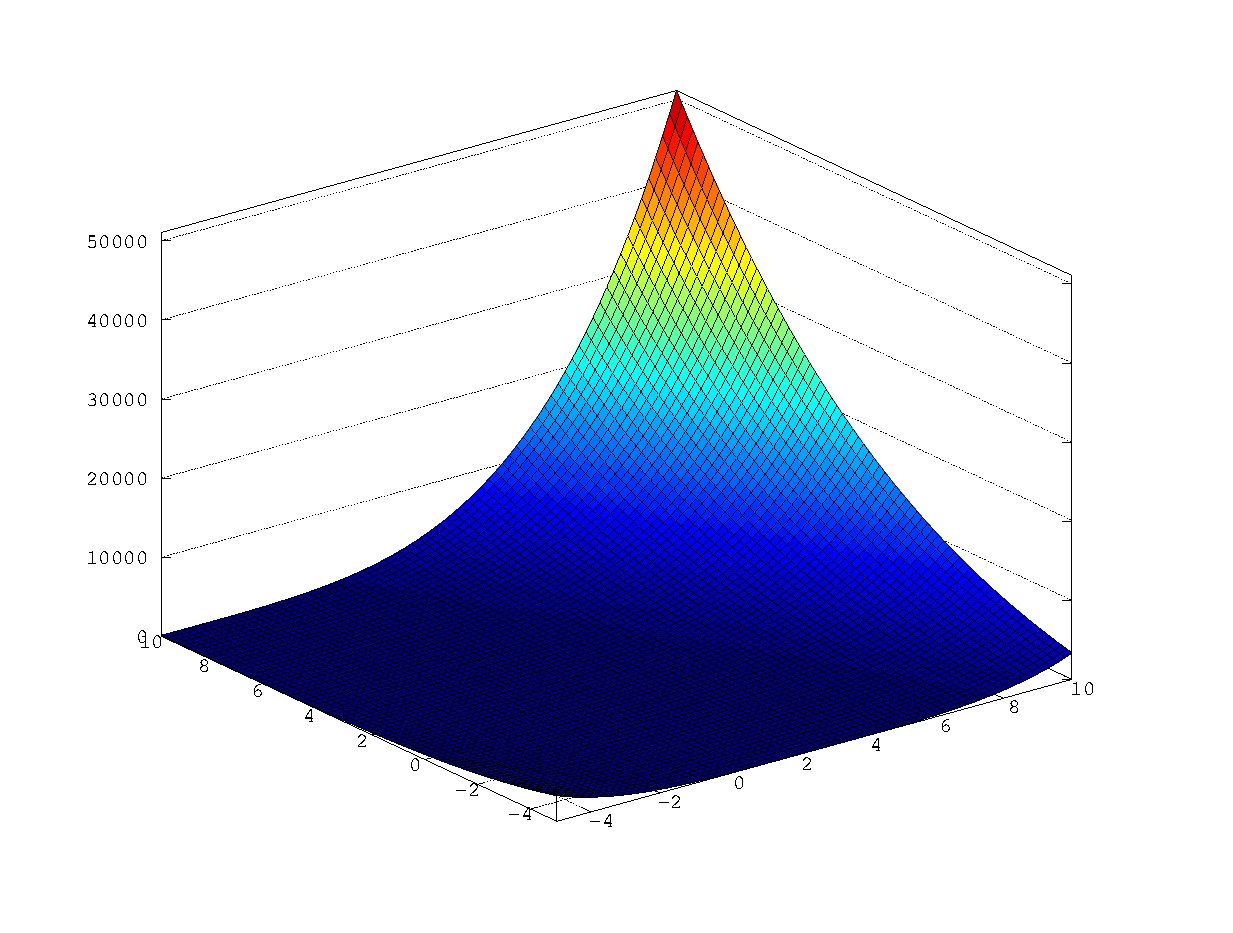
\includegraphics[width=\textwidth]{Images/Zakharov}
			\caption{Zakharov function [-5.0, 10.0].}
		\end{figure}

\end{document}
